\documentclass[12pt,a4paper]{article}
\usepackage{preamble}
\usepackage{graphicx}
\usepackage{fancyvrb}
\usepackage[bottom]{footmisc}
\newcommand\sessiontitle{Lab Session 2}
\newcommand\sessionsubtitle{Images, Histograms, Intensity clipping}

%%%%%%%%%%%%%%%%%%%%%%%%%%%%%%%%%%%%%%%%%%
\begin{document}

\section{Image IO (input/output)}
\label{task:io}
\begin{enumerate}
    \item Open VS Code in a GitHub Codespace (see Task 2 of Lab Session 1) using the repository which you created before (see Task 1 of Lab Session 1).
    \item Open the notebook \texttt{task2.ipynb}.
    \item Enter the following code into the \emph{first} code cell of the notebook and run it:
\begin{Verbatim}[frame=single]
import numpy
import matplotlib.pyplot as plt
\end{Verbatim}
    \textbf{Notes:}
    \begin{itemize}
        \item The first instruction should be clear from the lecture. The second instruction loads the module ``\texttt{matplotlib.pyplot}'' and makes it available by using the abbreviation ``\texttt{plt}''. This module is useful for visualizing data.
        \item Make sure this code cell \emph{always} remains the very first code cell of your notebook, so it is run first when the Notebook is re-run from top to bottom.
    \end{itemize}
    \item Then, extend the notebook as follows:
    \begin{enumerate}
        \item Use \texttt{img = plt.imread(\textquotesingle{}data/cells.png\textquotesingle)} to load an image. -- \textbf{Note:} The type of the returned object (\texttt{img}) is \texttt{numpy.ndarray} (also see the introduction on page~\pageref{sec:ndarray}). Objects of this type represent images.
        \item Use \texttt{plt.figure()} (or, e.g., \texttt{plt.figure(figsize=(15,8))} if you want to specify the size of the figure) to add a \emph{figure} to a code cell of the notebook. Then, \emph{within the same code cell}, use \texttt{plt.imshow(img, \textquotesingle{}gray\textquotesingle)}\footnote{The parameter ``\texttt{\textquotesingle{}gray\textquotesingle}x' in ``\texttt{plt.imshow(img, \textquotesingle{}gray\textquotesingle)}'' specifies the color map for a \emph{monochromatic} image (i.e.\ a two-dimensional array of image \emph{intensities}, non-RGB) for visualization (e.g., gray-scale)} to display the image within the figure. In addition, use \texttt{plt.colorbar()} after the \texttt{imshow}-instruction to include a legend of the gray-scale encoding. Run the code cell \emph{with and without} the \texttt{colorbar}-instruction and observe the differences. Finally, you should obtain an output like this:
        \begin{figure}[h!]
            \centering
            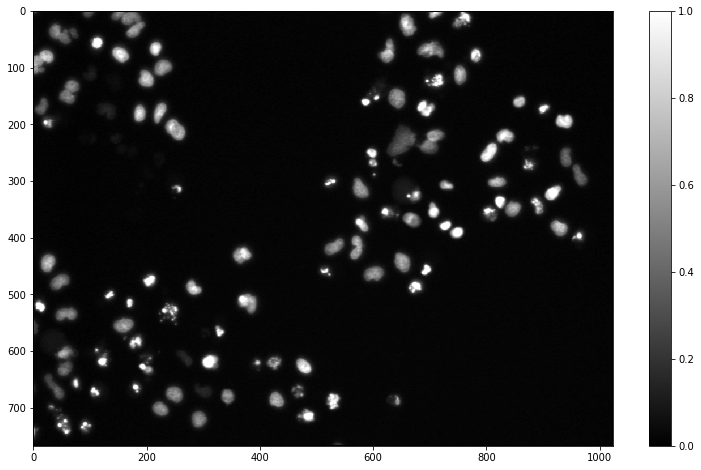
\includegraphics[width=0.5\textwidth]{images/task2-1.png}
        \end{figure}
    \end{enumerate}
\end{enumerate}

\section*{Introduction: Working with \texttt{numpy.ndarray} objects}
\label{sec:ndarray}
If \texttt{img} is an object of the type \texttt{numpy.ndarray}, then the object \texttt{img} has the following attributes and methods:
\begin{center}\begin{tabular}{p{0.46\textwidth}|p{0.48\textwidth}}
    \textbf{Attributes} (data) & \textbf{Methods} (behaviours) \\
    \hline
    \begin{description}[topsep=0pt,partopsep=0pt]
    \item[\texttt{img.ndim}:] Corresponds to the dimension of \texttt{img}.
    \item[\texttt{img.shape}:] If \texttt{img} is an image, then the element \texttt{img.shape[0]} corresponds to the image height (number of rows) and \texttt{img.shape[1]} to the image width (number of columns).%
    \end{description}%
    &
    \begin{description}[topsep=0pt,partopsep=0pt]
    \item[\texttt{img.copy()}:] Tells \texttt{img} to return a copy of itself.
    \item[\texttt{img.clip(t1, t2)}:] Tells \texttt{img} to return a copy of itself using intensity clipping (see Task~\ref{task:clipping}).
    \item[\texttt{img.flatten()}:] Tells \texttt{img} to return a flat representation of itself (see Task~\ref{task:histograms}).%
    \end{description}%
    \vskip1ex (Methods are like functions \emph{which belong to objects}.)
\end{tabular}\end{center}
Note that the above is \emph{not} a complete list (there are many more attributes/methods\footnote{see \url{https://docs.scipy.org/doc/numpy/reference/generated/numpy.ndarray.html}} which are \emph{not} relevant for this assignment).

\vskip2ex\noindent\textbf{Further hints regarding \texttt{numpy.ndarray} objects:}
\begin{enumerate}
    \item The pixel in the upper left corner of the image has the coordinates $(0,0)$, and the pixel in the lower right corner has the coordinate $(\text{width}-1, \text{height}-1)$.
    \item If \texttt{img} is an image (i.e.\ object of the type \texttt{numpy.ndarray}), then the intensity value of a pixel at position \texttt{p} corresponds to \texttt{img[p]}, where \texttt{p} has two elements (row, column). Alternatively, you can use \texttt{img[row, column]} instead of \texttt{img[p]}.
\end{enumerate}

\section{Histograms}
\label{task:histograms}
Extend your notebook by a histogram of the previously loaded image -- \textbf{Hints:}
\begin{enumerate}
    \item The function \texttt{plt.hist(data)} produces a histogram of a \emph{sequence of values} (\texttt{data}).
    \item In Python, a \emph{sequence} is, for example, a list, a \emph{flat} array, \ldots
    \item The image \texttt{img} is a \emph{two-dimensional} array and \texttt{img.flatten()} returns a flat representation (sequence of all pixel values).
\end{enumerate}

\begin{samepage}\section{Intensity clipping}
\label{task:clipping}
Given two thresholds $T_1$ and $T_2$, each pixel $x,y$ of the image with an intensity value $g\left(x,y\right)$ less than the threshold $T_1$ is assigned the value $T_1$ and each pixel with a value greater than $T_2$ is assigned the value $T_2$. Pixels with a value between the two thresholds $T_1$ and $T_2$ remain unchanged:
\begin{align*}
    g_\text{clip}\left(x,y\right) = \begin{cases}
        T_1 & \text{ if $g\left(x,y\right) < T_1$,} \\
        T_2 & \text{ if $g\left(x,y\right) > T_2$,} \\
        g\left(x,y\right) & \text{ otherwise}
    \end{cases}
\end{align*}
If $g$ is the image \texttt{img}, $y$ is the image \texttt{row}, and $x$ is the image \texttt{column}, then the mathematical expression $g\left(x,y\right)$ corresponds to \texttt{img[row, column]} in Python.

\vskip1ex In this task, you will \textbf{perform intensity clipping} (i.e.\ compute $g_\text{clip}$, in \emph{three} different ways) using the previously loaded image (Task~\ref{task:io}) and visualize the result using the \texttt{imshow} function.
\begin{enumerate}
    \item Perform intensity clipping using the method \texttt{clip} of \texttt{numpy.ndarray}.
    \item Reproduce the behaviour of the method \texttt{clip}, i.e.\ perform intensity clipping \emph{without} using the method \texttt{clip}!
    \begin{enumerate}
        \item Use \emph{two} nested \texttt{for}-loops (one outer loop for the image rows or columns, one inner loop for the pixels of the current row/column) and \texttt{if}-conditions.
        \item Use a \emph{single} \texttt{for}-loop and \texttt{if}-conditions -- \textbf{Hint:} \texttt{numpy.ndindex(img.shape)} yields an iterable. The items of this iterable correspond to \emph{all} pixel coordinates of the image  \texttt{img}. Each item is a pair of coordinates (i.e.\ row and column). Use ``\texttt{[0]}'' and ``\texttt{[1]}'' to access the corresponding row and column of an item.
    \end{enumerate}
\end{enumerate}
Include a legend of the gray-scale encoding (using ``\texttt{plt.colorbar()}'') in \emph{each} figure!\end{samepage}

\section{Writing re-usable code \bonustask}
\label{task:functions}
In the previous task, you have used loops to reproduce the behaviour of the method \texttt{clip} of \texttt{numpy.ndarray}. Now, make this code \emph{re-usable} by putting it into a \emph{function} which you can use anytime later. For your convenience, a skeleton of the code you need to write to implement the function is already added to the notebook (see ``\texttt{def clip\_image}\ldots'').

\end{document}
